\section{Course Overview}

ME 533: Machine Design is a lecture based class that focuses on stress/strain analysis, load determination,
and failure theories. Despite being the first machine design class in the mechanical engineering curriculum, 
the material is a continuation of topics covered in two required civil engineering courses: CE 333: Statics
and CE 533: Mechanics of Materials.

As a higher level course that relies on well established theories and analysis methods, machine design
presents several oppurtunities for programmatic solutions to problems, though Excel calculators may
be more appropriate in some cases. Despite this, machine design does not require programming for 
assignments or projects, those this fact has varied depending on the current instructor. 

Homeworks typically involve resolving loads on various members, analyzing the internal stresses, and 
determining the safety of a design using the appropriate failure theories. When appropriate, deformation
plots are drawn to highlight points of failure. The class finishes with discussions on spring and fastener
design, which involves heavy iteration.

\section{New Tool for Assignments}

Since no assignments currently make use of programming, two homework questions have been solved to demonstrate
potential uses for programming in the course. Rather than writing a Python script to solve iterative design or
strictly numerical probems (see chapters on Thermodynamics, Fluid Mechanics, or Heat Transfer for examples of
this), both questions focus on finding and plotting beam deflection using singularity functions. 

The most simple adoption of programming into singularity function assignments would be requiring computer
generated plots. Students would first solve for reaction forces, create a singularity equation, integrate
several times, and then create a plot using the deformation equation. The solution presented here takes a 
higher level approach by accepting the loading forces on the bar and then creating and integrating the 
singularity equation automatically. This is done through a graphical user interface developed and executed
in Python.

The GUI can be launched in Python (with the code provided in the associated GitHub repository) or through
the terminal as a Python module. Once launched, the application will open in a new window, which is shown
in Figure \ref{fig:singularity-gui}. The home page contains instructions for using the solver, so the details 
here will be sparing. The second page is dedicated to beam configuration, including legnth, cross section, 
material, and boundary conditions. The next page presents various forms of loading to add
to the beam. The last page allows custom materials to be added to the list of materials.

\begin{figure}[h]
    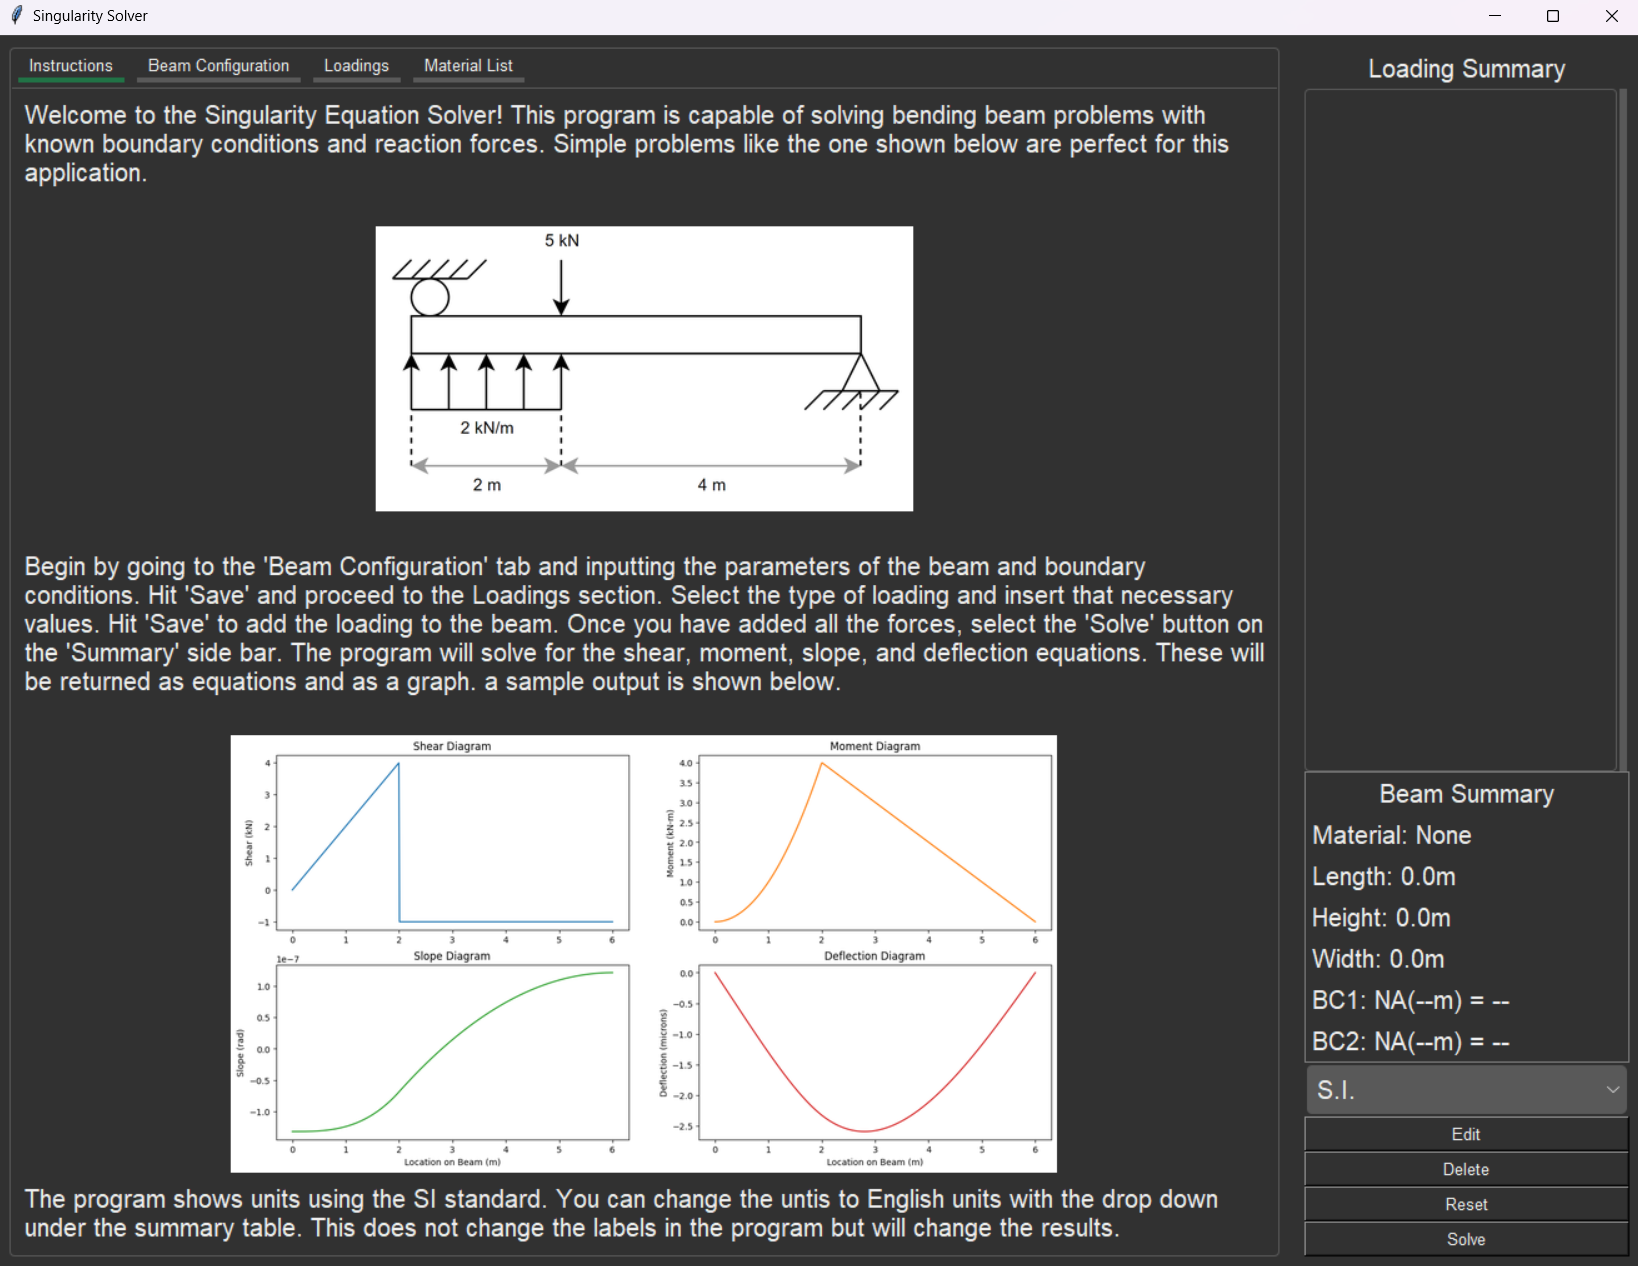
\includegraphics[width=\textwidth]{singularity-gui.png}
    \centering
    \caption{Singularity Solver GUI}
    \centering
    \label{fig:singularity-gui}
\end{figure}

While the GUI currently automates significant portions of singularity problems, several features should be
added at a later date, including non-rectangular cross sections (though a work around is presented) and
the ability to add supports to the beam. This would give the program the ability to calculate the reaction
forces and deterine boundary conditions without relying on the user to correctly find and input them.

Since this application takes most of the work out of the hands of the students, it would not be a good tool
for teaching singularity functions. Rather, the application would be best utilized in when finding the shear,
moment, slope, or deformation of a beam is one part in the context of a larger problem. Additionally, 
it would serve as a realistic look at how most analysis is done in industry - by a computer.

\section{Project Deliverables}

In the GitHub repository associated with this paper, which can be found in Appendix \ref{appendix:appendix_github},
the folder titled ``machine-design'' contains both the problem statements and solution guides for the two questions
introduced in the previous section. The folder also contains a README that details what is in each file and 
what software is needed to complete the assignments. 

For these projects to be added to the class, the instructor would  need to give the skeleton files to 
students as a problem statement and the MNE folder as Python library. Using one of the two questions as an in-class
example would serve as a good oppurtunity to remind students how to use Python with Jupyter Notebooks and to 
demonstrate how to open and use the singularity function GUI.
